\documentclass{article}
\usepackage[utf8]{inputenc}
\textheight = 25cm 
\textwidth = 15cm
\topmargin = -3.0cm 
\oddsidemargin = 1.5cm
\usepackage{hyperref}
\hypersetup{
    colorlinks=true,
    linkcolor=blue,
    filecolor=blue,
    citecolor=black,      
    urlcolor=blue,
    }

\usepackage{float}
\usepackage{graphicx}

\usepackage{gensymb}

\usepackage{amsmath}
\usepackage{amssymb}
\usepackage{amsfonts}
\usepackage{mathtools, xparse}
\usepackage[shortlabels]{enumitem}

\usepackage[many]{tcolorbox}
\usepackage{lipsum}
\usepackage{amssymb}

\title{Cuestionario 2 Termodinámica}
\author{Cerritos Lira, Carlos}
\date{18 de Mayo del 2020}

\newcommand{\pr}[1]{\left(#1\right)}
\newcommand{\pt}[2]{\dfrac{\partial #1}{\partial #2}}

\begin{document}
\maketitle
\section*{1.-}
Una olla está llena a la mitad con agua y se tapa formando un sello
hermético que no permite el escape de vapor. La olla se calienta en una estufa 
formándose vapor de agua dentro de ella La estufa se apaga y el vapor se condensa. 
¿Este ciclo es reversible o irreversible?. Explique
\begin{tcolorbox}[breakable]
    Irreversible, ya que tendría que ocurrir que el agua recuperara su temperatura de forma 
    espontanea para volver al estado de vapor.
\end{tcolorbox}

\section*{2.-}
Convertir energía mecánica totalmente en calor, ¿Viola la segunda ley de la termodinámica?
¿Y convertir calor totalemtne en trabajo? Explique.
\begin{tcolorbox}[breakable]
    De acuerdo al segundo axioma a la Planck: \textit{No existe nignuna transformación termodinámica
    cuyo único resultado sea la abosrción de calor de un solo foco y la producción de una cantidad
    equivalente de trabajo}. \\ \\
    Efectivamente, toda la energía mecánica puede transformarse en calor, un ejemplo de esto puede ser cuando se 
    usa el freno de mano en un auto, también podemos relacionar esto con el concepto de la degradación de la energía. \\ \\
    Por otra parte no podemos transformar todo el calor en trabajo, ya que entonces tendríamos una 
    máquina con eficiencia 1, lo que contradice el axioma de Planck.
\end{tcolorbox}

\section*{3.-}
\begin{enumerate}[a)]
    \item Si ninguna máquina real puede ser tan eficiente como una máquina de Carnot que opera entre las mismas 
    temperaturas ¿qué sentido tiene deducir y analizar la ecuación $\rho = 1- \frac{T_C}{T_H}$?
    \item ¿Qué eficiencia tendría una máquina de Carnot que opera con $T_H = T_C$?,
    ¿Y si $T_C=0K$ y $T_H$ cualquier otra temperaturas mayor? Discuta. 
\end{enumerate}
\begin{tcolorbox}[breakable]
    \subsubsection*{a)}
    Nos sirve como un referente para comparar que tan eficiente es una máquina real comparada con la 
    mejor eficiencia que se puede obtener de forma ideal.
    \subsubsection*{b)}
    Cuando $T_H = T_C$ se tiene:
    \[ \rho = 0\]
    Como no hay una diferencia de temperatura entre las fuentes no se puede realizar un trabajo, 
    por lo tanto la eficiencia es cero. \\ 
    Cuando $T_C=0K$ se tiene:
    \[ \rho = 1 \]
    Todo el calor se convierte en trabajo, situación poco ideal de implementar pues conseguir 
    temperaturas bajas es costoso.
\end{tcolorbox}

\section*{4.-}
Visalice el ciclo de Carnot para un Gas Ideal y discuta cuales serían las consecuencias de que dos isotermas 
se cortaran o que dos adiabáticas se cortaran.
\begin{tcolorbox}[breakable]
    El Ciclo de Carnot para un gas ideal se puede visualizar con el diagrama $PV$ y consta de 4 procesos:
    \begin{itemize}
        \item Dos segmentos adiabáticos.
        \item Dos segmentos isotérmicos a temperatruas $T_H$ y $T_C$.
    \end{itemize}
    \begin{figure}[H]
        \centering
        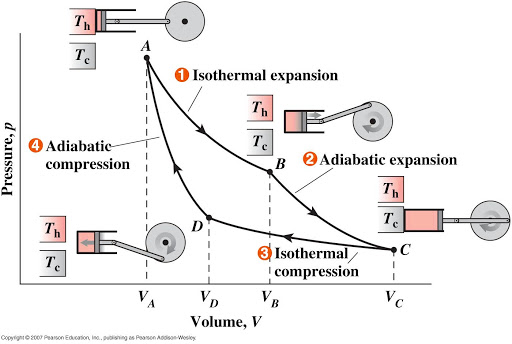
\includegraphics[scale=0.5]{images/p4_diagram.jpg}
    \end{figure}
    Si dos isótermas se cruzan podriamos crear una proceso de Carnot que funcione con un solo foco, lo cual es
    imposible
\end{tcolorbox}

\section*{5.-}
Demuestre que "Todos los motores reversibles que funcionan entre el mismo 
par de focos térmicos tienen la misma eficiencia térmica".
\begin{tcolorbox}[breakable]
    Supongamos que existen dos motores reverisbles $A$, $B$ que funcionan entre el mismo 
    par de focos térmicos con $\rho_A > \rho_B$. \\ \\
    Acomplamos los motores transformando a $B$ en un refrigerador ya que es un motor reversible, 
    además tenemos:
    \begin{align*}
        \rho_A &> \rho B \\
        \frac{W_A}{Q} &> \frac{W_B}{Q} \\
        W_A &> W_B
    \end{align*}
    $W_A > W_B$, por lo tanto $A$ puede proporcionar el trabajo necesario,
    tenemos el siguiente diagrama:  
    \begin{figure}[H]
        \centering
        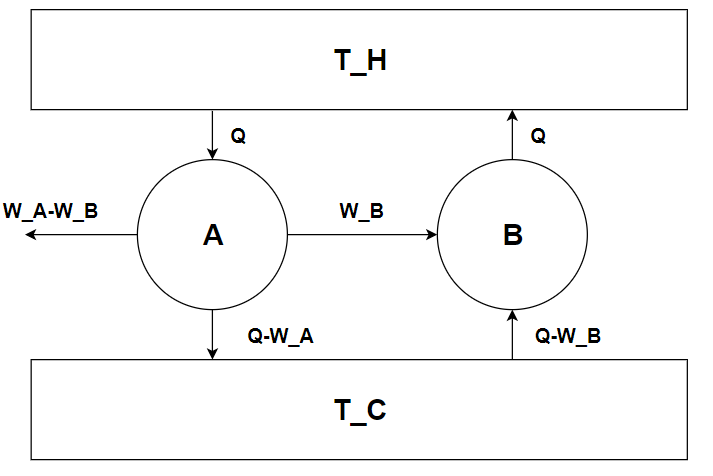
\includegraphics[scale=0.5]{images/p5_diagram.png}
        \caption{Diagrama acoplamiento de motores}
        \label{}
    \end{figure}
    Este nuevo motor toma un calor:
    \[ Q_T = Q-W_B-(Q-W_A) = W_A - W_B \]
    de la fuente $T_C$ y genera un trabajo: 
    \[ W_T = W_A-W_B \]
    Esto viola el segundo axioma de Planck ya que tomamos una cantidad $Q_T$ del un solo foco
    y producimos la misma cantidad de trabajo. \\ \\
    Por lo tanto no existen dos motores reversibles $A$,$B$ tales que $W_A > W_B$, esto es 
    todos los motores reversibles tienen la misma eficiencia.
\end{tcolorbox}



\end{document}